% This is LLNCS.DOC the documentation file of
% the LaTeX2e class from Springer-Verlag
% for Lecture Notes in Computer Science, version 2.4
% \documentclass{llncs}
\documentclass[citeauthoryear]{llncs}
\usepackage{llncsdoc}
%

\markboth{Orbione-Bot Team Description Paper}{Lera et al.}

\def\addtocontents#1#2{}%
\def\addcontentsline#1#2#3{}%
\def\markboth#1#2{}%


\usepackage[pdftex]{graphicx}
\graphicspath{{figures/}}
\DeclareGraphicsExtensions{.pdf,.jpeg,.png}
  
  
\begin{document}
\title{Orbione-Bot 2016 Team Description Paper }

\author{Francisco J. Rodr\'iguez Lera, Fernando Casado, Jes\'us Balsa, Vicente Matell\'an\inst{1} \and Francisco Mart\'in Rico\inst{2}}

\institute{Universidad de Le\'on, 24071, Le\'on, Spain
\and
Universidad Rey Juan Carlos, Madrid, Spain}

\titlerunning  \toctitle
\authorrunning \tocauthor

\maketitle
%
\begin{abstract}
This report aims to show the capabilities of the Spanish team named Orbione-Bot gathered to participate in the RoboCup@Home competition. It shows the background of our team members, the robot that we will be used (RB1) and the contributions to the RoboCup@Home goals that we are expecting. It also describes our software architecture the visual object recognition system, our autonomous navigation based on RGB-D sensors, the dialogue module that includes context awareness, and the mobile manipulation abilities. These components have been tested in periodically open demonstrations held in our lab where we have built a mock-up apartment. 

\end{abstract}
%
\section{Introduction}


The research goal of our team is how to create more acceptable socially assistive robots. RoboCup@Home competition will let us validate our results by external reviewers, and contrast them with other teams' ideas,  before deploying them in real home environments, and after testing them in our mock-up home.

The background of our team in robotic competition is the Watermelon Project. This project was initiated at at the University Le\'on's  Robotics Group in 2012. In 2013  the Universidad Rey Juan Carlos's robotic group joined the team. 


%\subsection{Background}

%Our original goal was to create a ultra-low cost robotic platform that could enter robotic competitions. We propose it as an starter kit for robotics researchers willing to participate in robotics competitions like RoCKIn. The RoCKIn 2014 events allowed us to test our approach intensively, which generated several improvements in our robot. This robot can be used in the labs for researching and for analyzing semi-autonomous behaviors in  real homes. 

MYRA - Mayores y Realidad Aumentada in Spanish (''Elderly and Augmented Reality'' in English) was the code name given to the original project more than two years ago. The main goal was to build an assistance robotics platform that would be suited to the needs of old people, such as helping them to take the right medication at the right time. We intended to study the human-robot interaction using augmented reality, and a target demographic with usually little experience with robots or technology overall. 

The Watermelon team was established at the end of 2013, in order to participate in the RoCKIn@Home camp that was going to take place in Rome on January the next year. Since the first moment, we focused our efforts on adding new software and hardware solutions, or improving the existing ones, in order to adapt MYRA for the
competition. Thus the MYRABot robot  \cite{martin2014myrabot} was created, and it has been continuously reshaped ever since.


\section{Hardware Platforms}

Our team will enter 2016 competition using RB1 (see figure~\ref{fig:rb1}). It is a mobile manipulator built by Robotnik.

\begin{figure*}[ht]
  \centering
  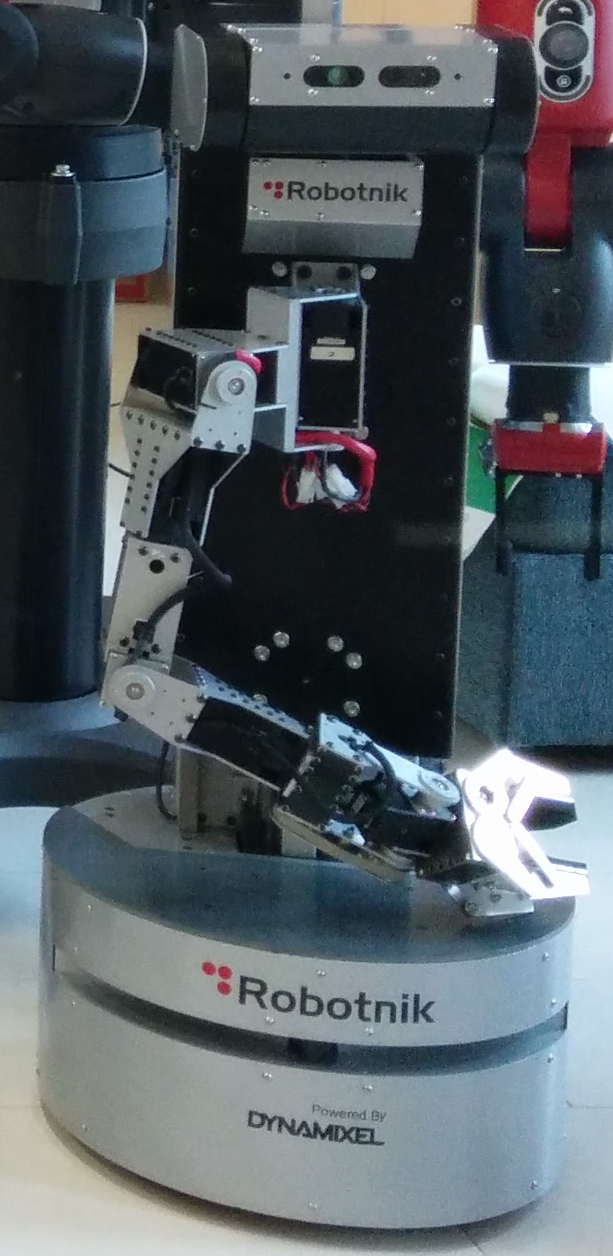
\includegraphics[width=0.3\textwidth]{rb1.png}
  \caption{RB1 platform}
  \label{fig:rb1}
\end{figure*}


We are also working in a bimanipulator plaftorm.



\subsection{Architecture}

We have a three layers architecture based on ROS and {BICA}~\cite{aguero2010behavior}. 
The lower layer corresponds to ROS, and is in charge of hardware management. 
The intermediate layer provides the robot skills in order to carry out specific duties (perception, navigation,...).

\begin{figure*}[ht]
  \centering
  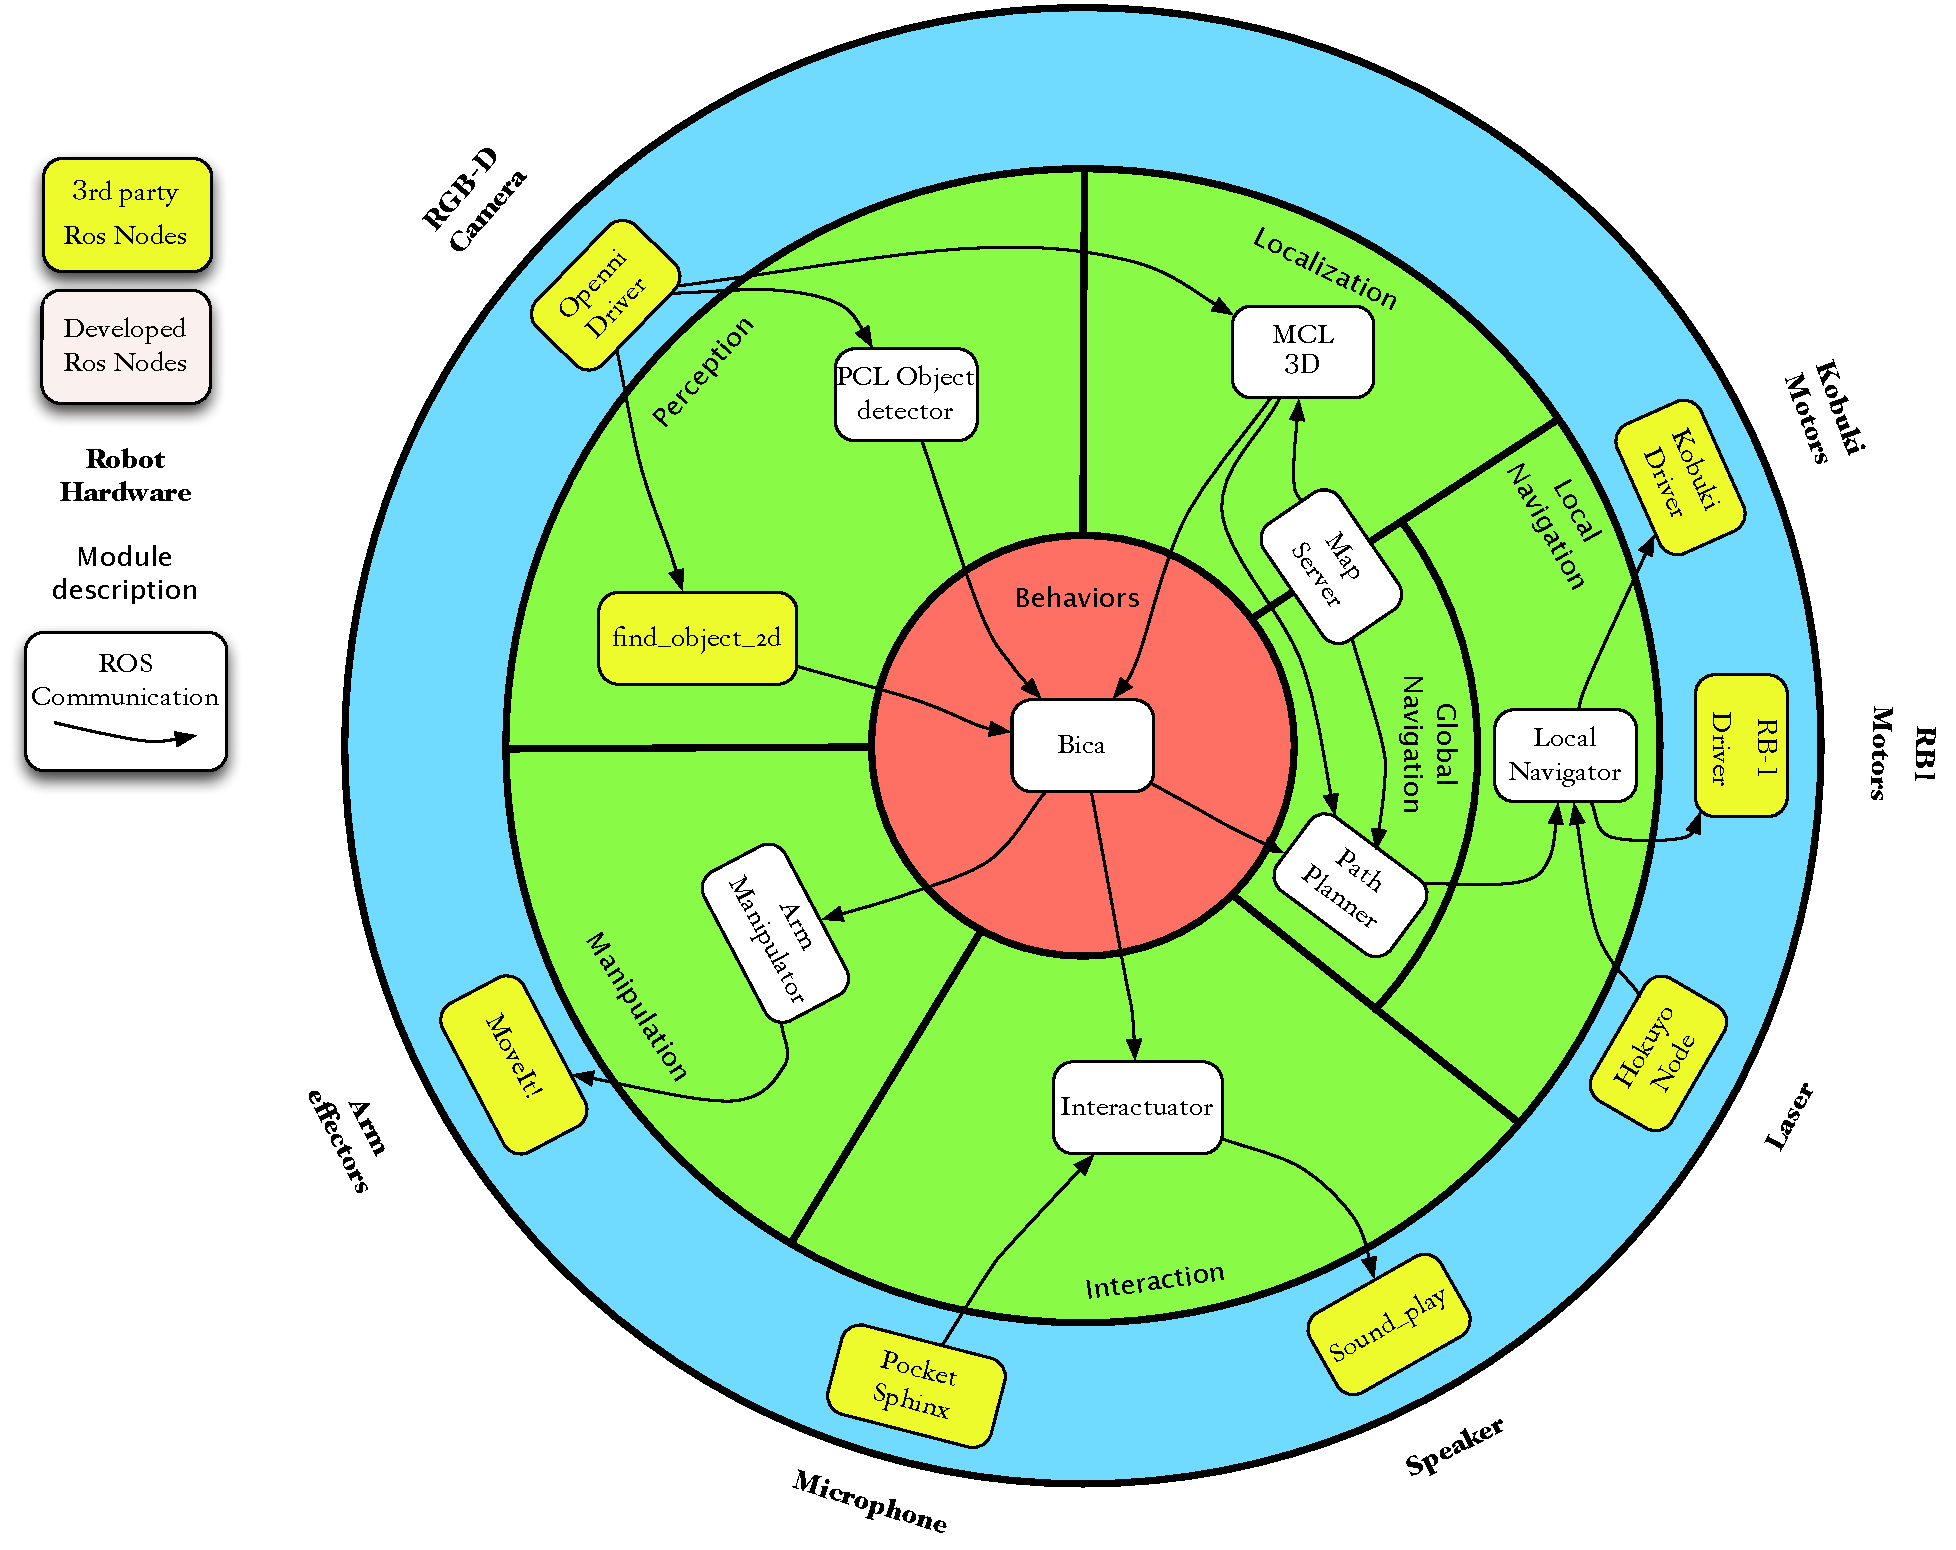
\includegraphics[width=0.8\textwidth]{rokinarq-142}
  \caption{Software architecture for RoCKIn competition.} 
  \label{fig:architecture}
\end{figure*}

The top layer presents {BICA}. It is a component-based for generating behavior s architecture. This node coordinates the various
capabilities of the robot depending on the task to be carried out by the robot.
Figure~\ref{fig:architecture} shows the overall architecture of the software we have developed for participating in the RoCKIn competition. 
% In the peripheral layer, which represents the hardware access, we
% use third-party ROS nodes. In the intermediate layer, we have developed the skills that should
% have the robot to carry out their duties. Bica is at the core of this architecture. 







\subsubsection{Component-based Architecture for Behaviour Generation}

We use a component-based architecture~\cite{aguero2010behavior} to generate robot behaviour s. We recently
started the integration of this approach to our platform for avoiding big and complex finite
state machines (FSMs) developed ad-hoc in each ROS node. 
% 
% Figure~\ref{fig:BicaandROS} describes the implementation scheme of a robotic application using our approach.
% There can be multiple ROS nodes containing components of our architecture, which communicate
% with other ROS regular nodes. Besides ROS communications, ICE can be used to
% interconnect any component with other processes or even to debug graphics applications.
% 
% 
% 
% \begin{figure}[ht!]
%   \centering
%   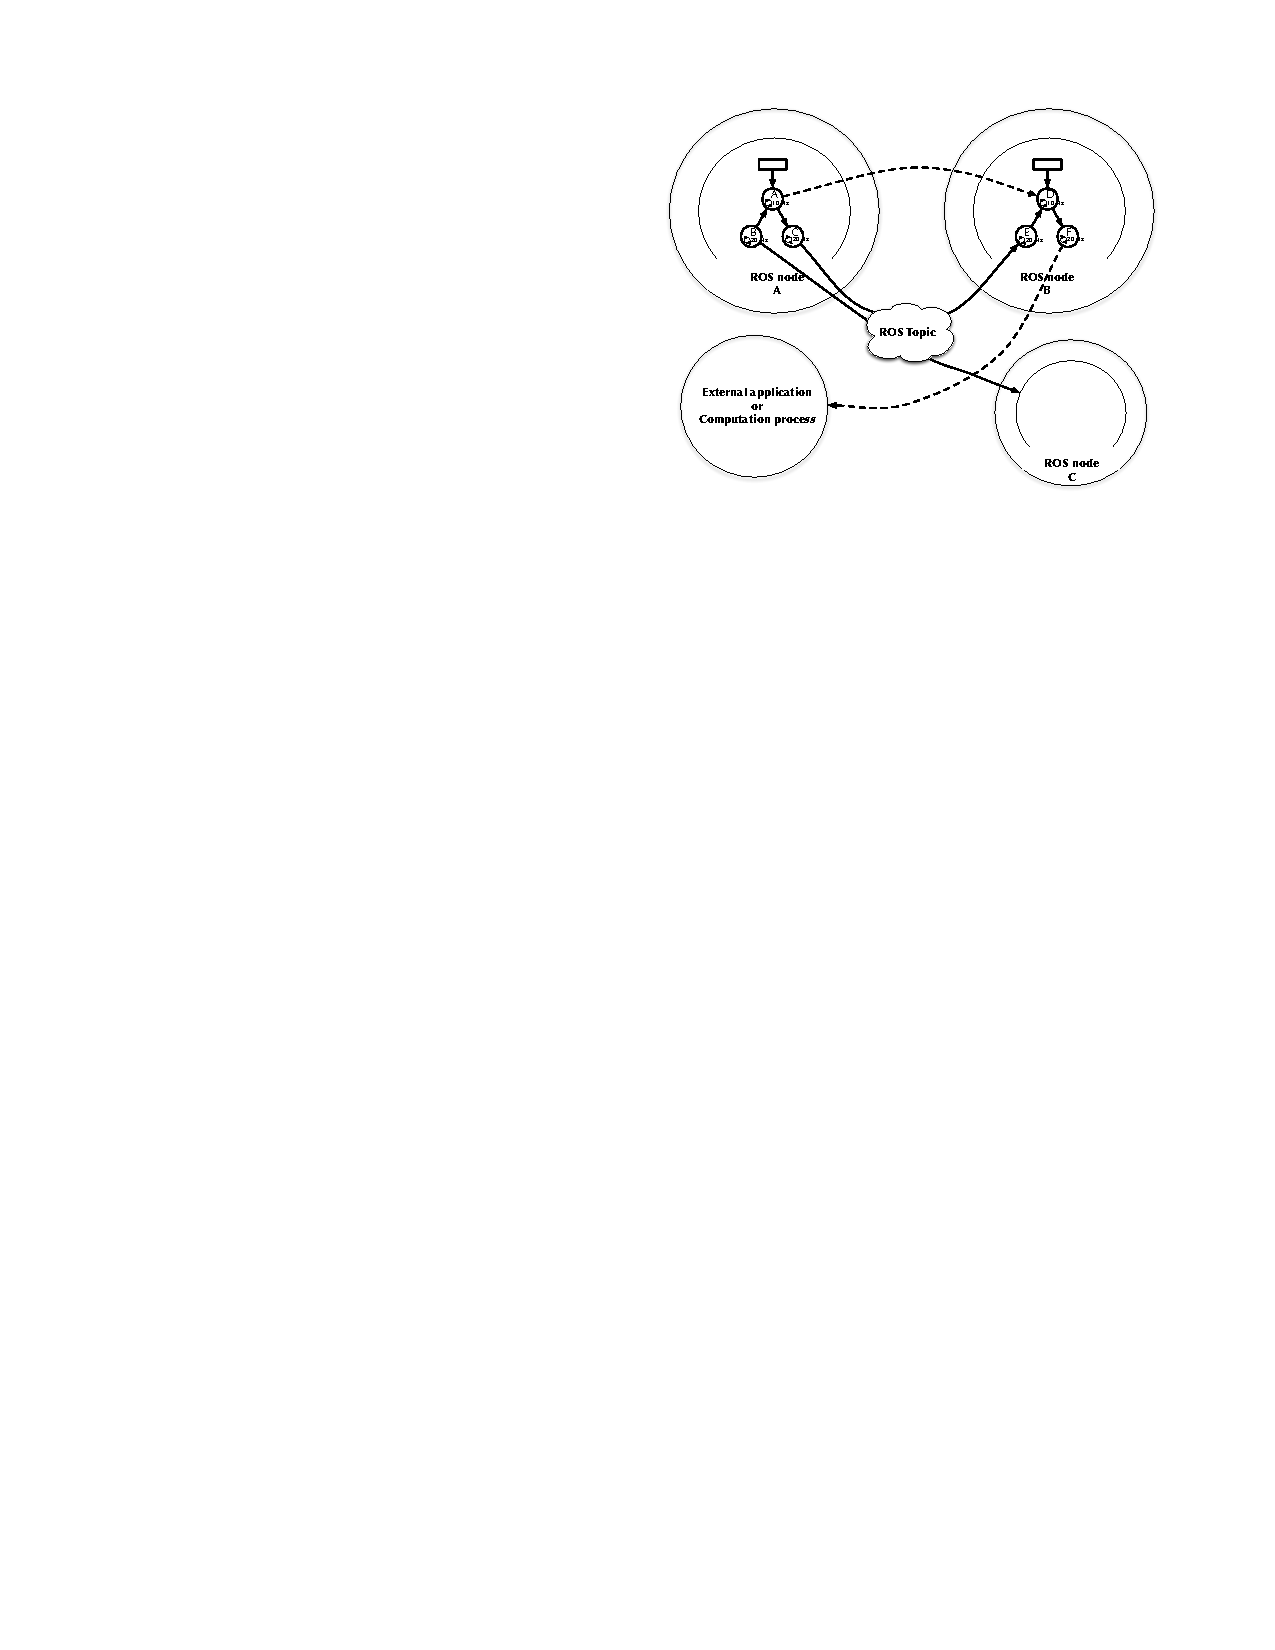
\includegraphics[width=0.5\textwidth]{50}
%   \caption{Bica implementation inside ROS nodes. Solid lines represent ROS communication, and dashed lines ICE.} 
%   \label{fig:BicaandROS}
% \end{figure}
% 



The basic functional unit in our architecture is the Component, simple functional units
that are executed iteratively at different rates. The main idea is to define components that
perform just a single task, but very efficiently. A running component can activate other
components, forming a dynamic hierarchy of components that implement a complete
behaviour .

Components can be very simple or very complex. Simple components communicate with
the underlying system methods to use sensors or motors, or some other components.
Complex components can be implemented as a FSM, so the set of components that are
activated depends of the current state.


Our approach uses only the required resources for a given task. When a component needs
another, it explicitly calls its step() method. Components that are not being used by
another component do not run, saving computing resources. 

We have developed a useful tool to design these complex components. This tool generates
the skeleton code for a behaviour  modelled graphically. Figure~\ref{fig:Bicacomponent} shows the implementation
of a component as an FSM with nine states (yellow circles). In each state, another component
(blue circles) are activated. From any component you can perform any communication with
other nodes ROS.


\begin{figure}[ht]
  \centering
  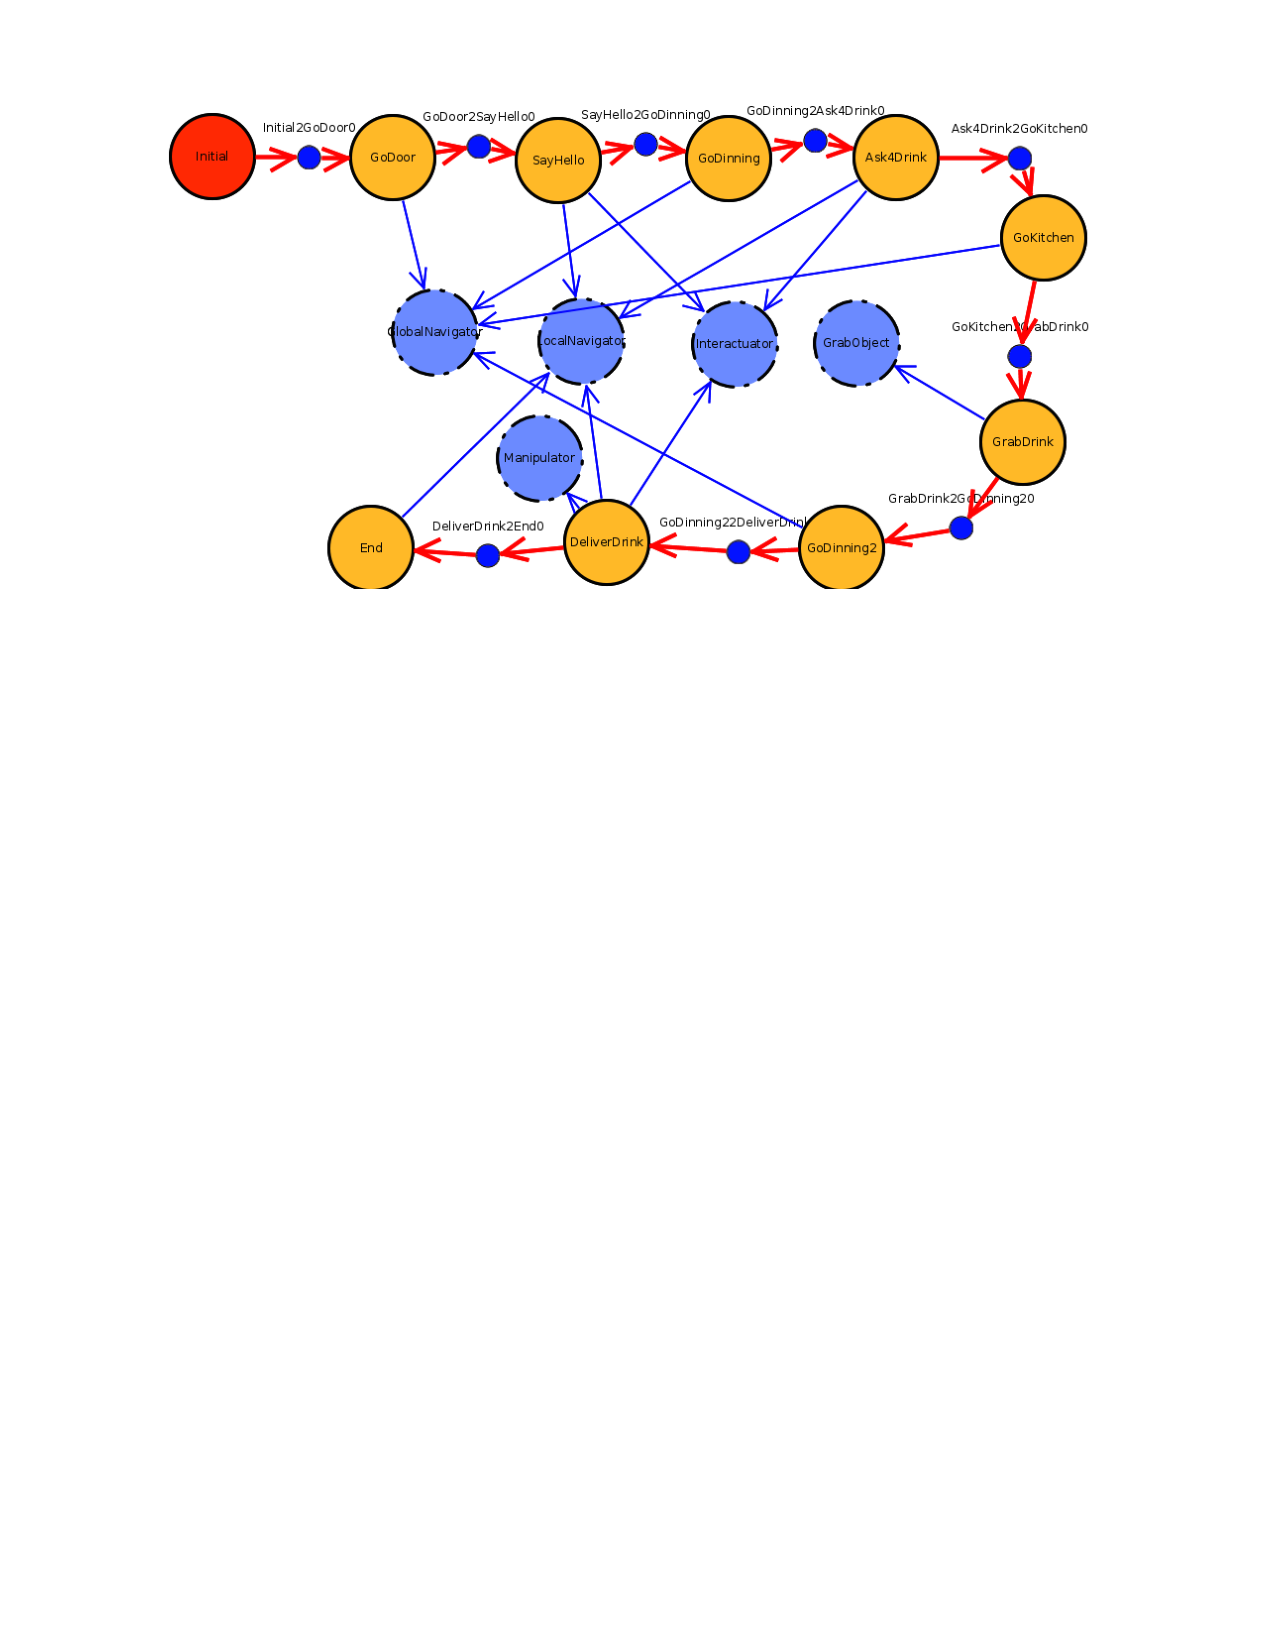
\includegraphics[width=0.5\textwidth]{202}
  \caption{Bica component implementing a finite state machine to define a high-level behaviour.} 
  \label{fig:Bicacomponent}
\end{figure}




\subsection{3D SLAM}

We use our own self-localization algorithm based on 3D perception. 
Our approach consists of creating a 3D map of a cloud formed by RGB-D or ColorOctomap \cite{hornung2013octomap} points. 
When the robot is running, we use an algorithm to contrast the MCL RGB-D perception with the map to evaluate the population of particles.
\begin{figure}[ht]
    \centering
    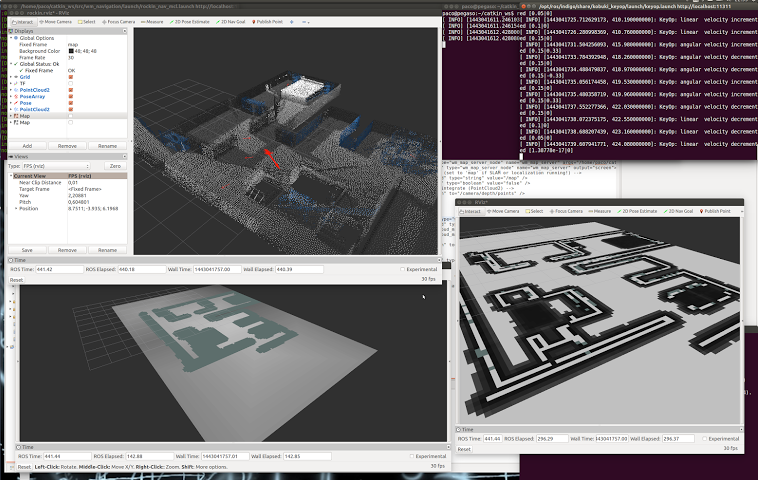
\includegraphics[width=.65\textwidth]{Navigation}
    \caption{Rviz and Gazebo running the first approach of our 3D visual navigation method.}
  \label{fig:navigation}
\end{figure}


\subsection{Context Awareness}


Context-awareness is a fundamental component in human robot interaction. Understanding the user activity context the robot improves the overall decision-making process. This is because, given a context, the robot can reduce the set of  feasible actions. 
We consider that using an on-board microphone and gathering environmental sounds we can improve the context recognition.

For this purpose, we have designed, developed and tested  a computational lightweight Environment Recognition Component (ERC). %In this iteration our ERC  is able to recognize a set of four home bells.
This component provides information to a Context-Awareness Component (CAC) that implements a hierarchical Bayesian network to tag user's activities based on the American Occupational Therapy Association (AOTA)  classification. 



The system implemented for real environment deployment  works as follows: 
\begin{enumerate}
 \item The robot analyzes on runtime the environment situation and processes a set of observations. 
 \item For simplifying, the solution links each observation with only one action \& operation. It makes that our four-layer solution became a three layers one.% which identifies the user activity.
 \item With this information the robot calculates the conditional probability of an activity given an observation $P(A|o)$ instead of the action \& operation nodes. 
 \item The conditional probability of the occupation nodes is defined by the associated activity  $P(Oc|a)$.
%  \item With this information the robot calculates the conditional probability $P(Oc|a)$.
\end{enumerate}


\begin{figure}[ht]
    \centering
    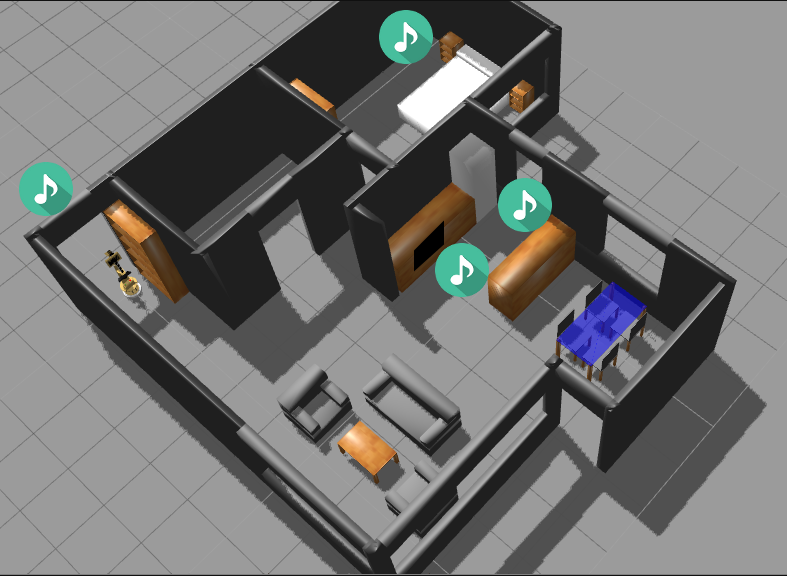
\includegraphics[width=.6\textwidth]{SimulatorContext}
    \caption{There are different acoustic singals available in all the real environments: doorbell, oven, fridge, ...}
  \label{fig:contextsimulator}
\end{figure}




\subsection{Social Navigation}

Navigating in a socially acceptable way is an important ability for mobile robots in populated
environments that requires efficiently detecting and tracking humans to negotiate the space with.
In particular, walking side by side is not a trivial problem that involves relative positioning
calculations to the accompanying person taking into account the environment limitations (narrow
corridors, turnings, etc.) as well as keeping its track towards its destination.


\begin{figure}[ht]
    \centering
    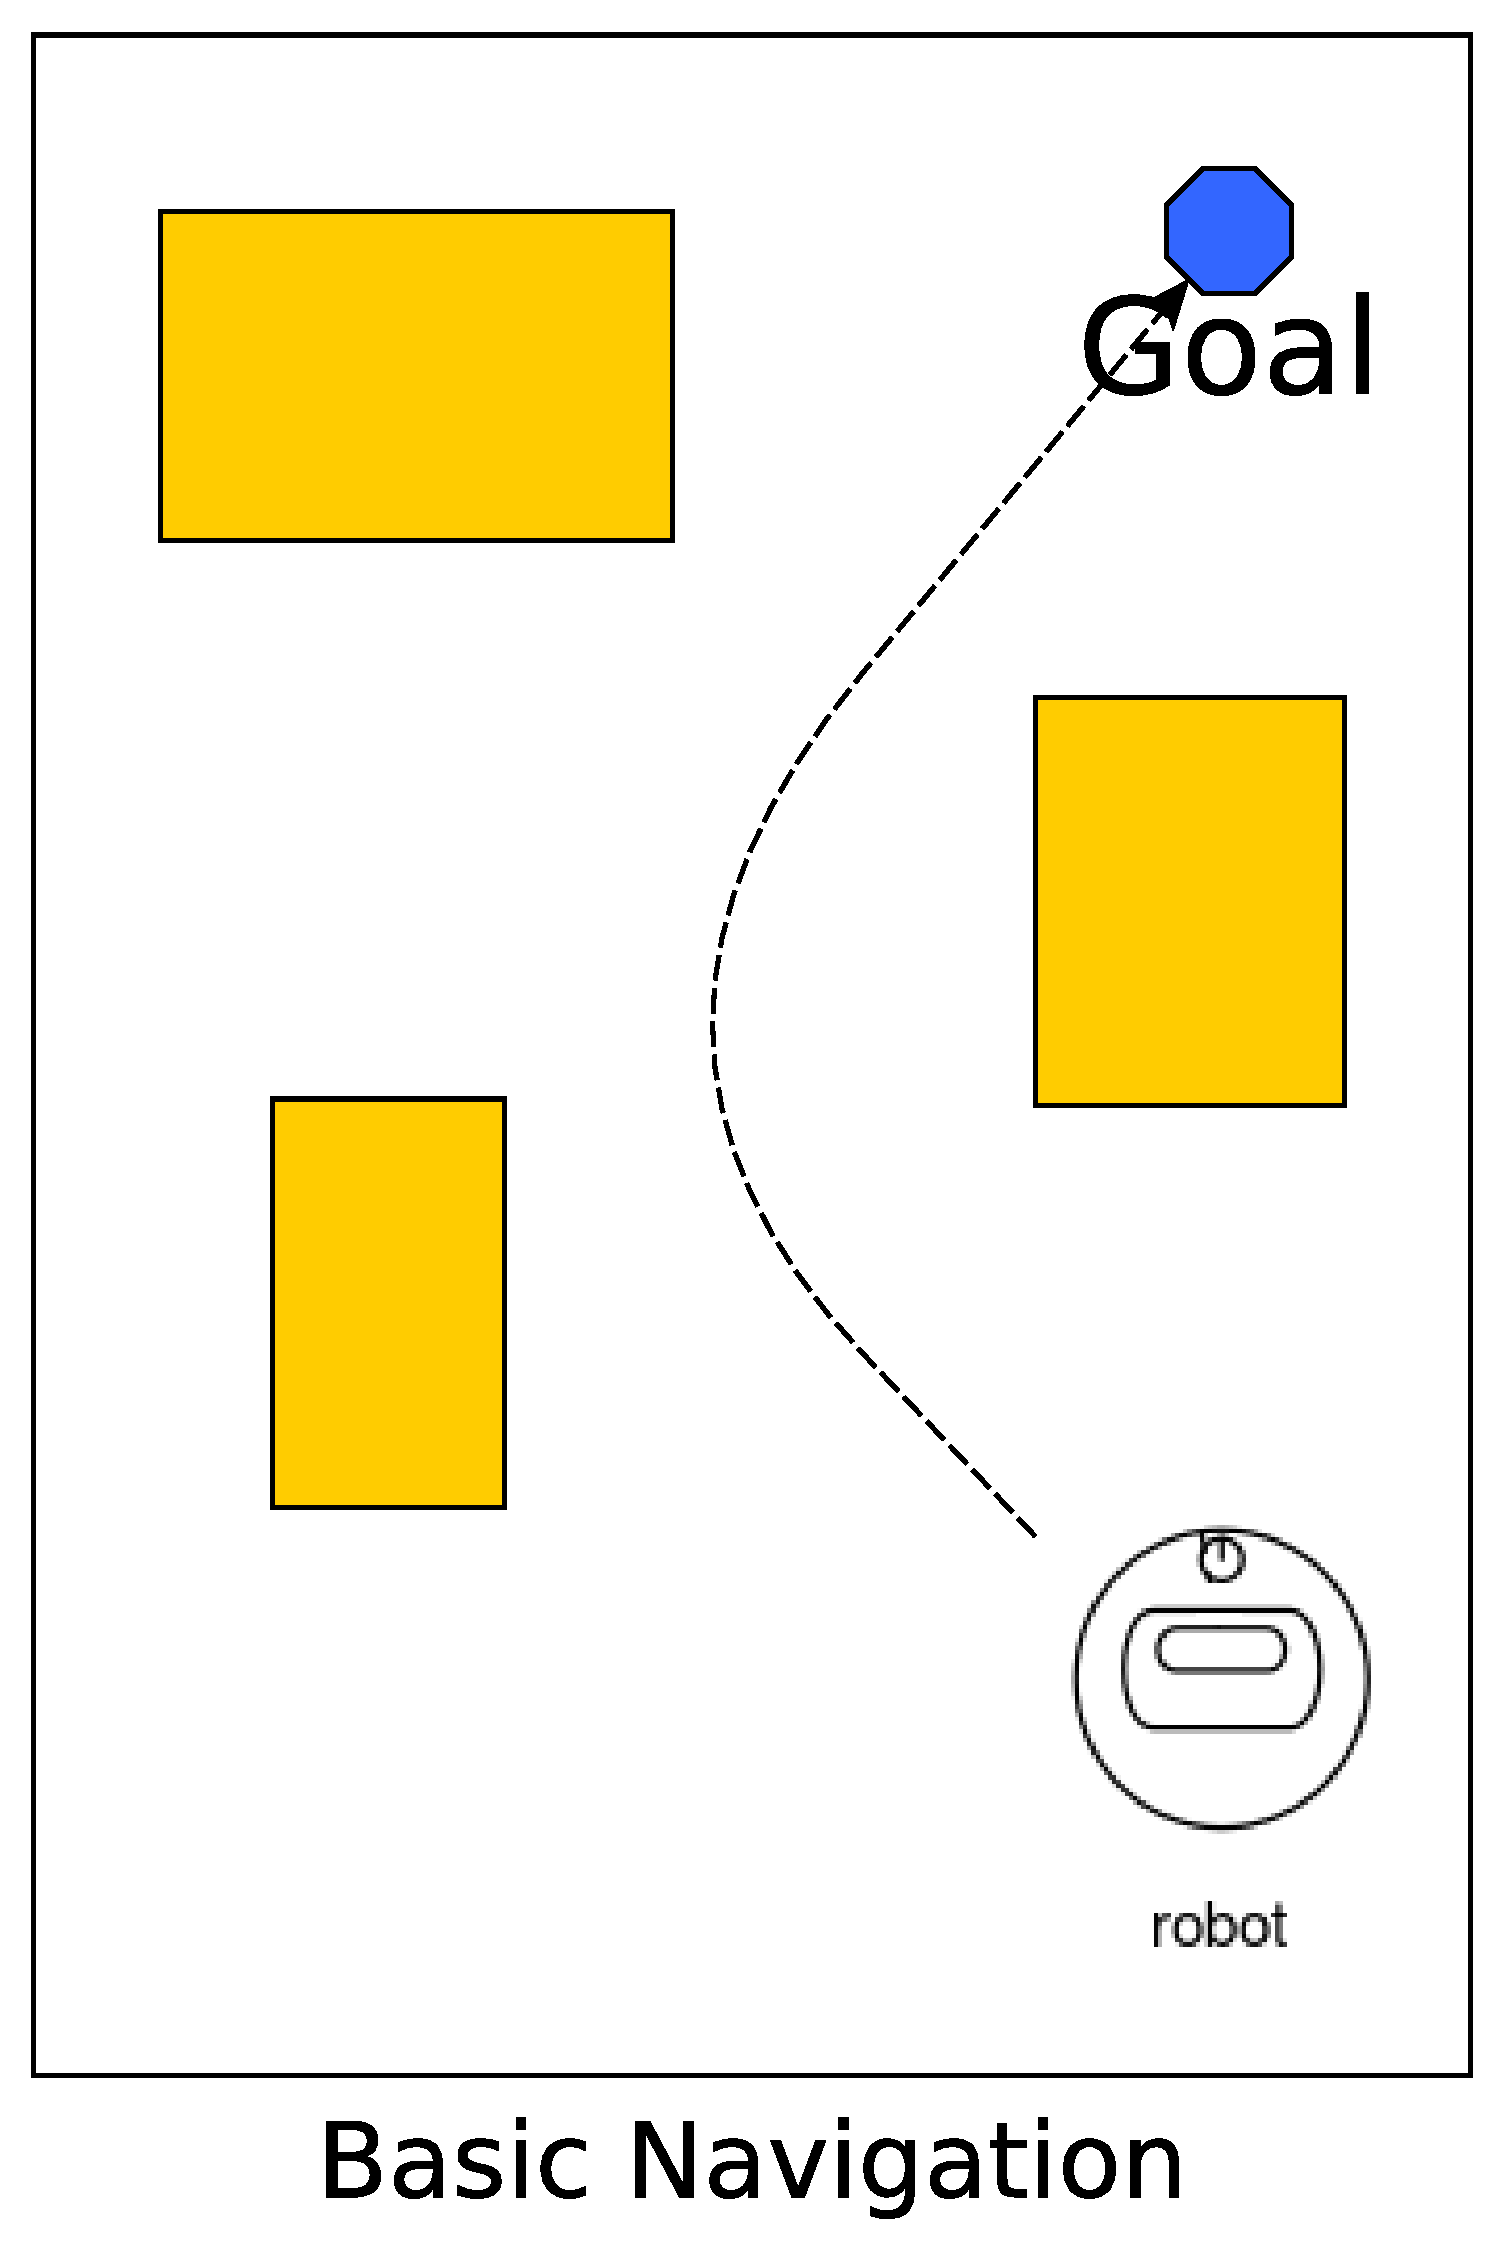
\includegraphics[width=.2\textwidth]{CasoBase}
    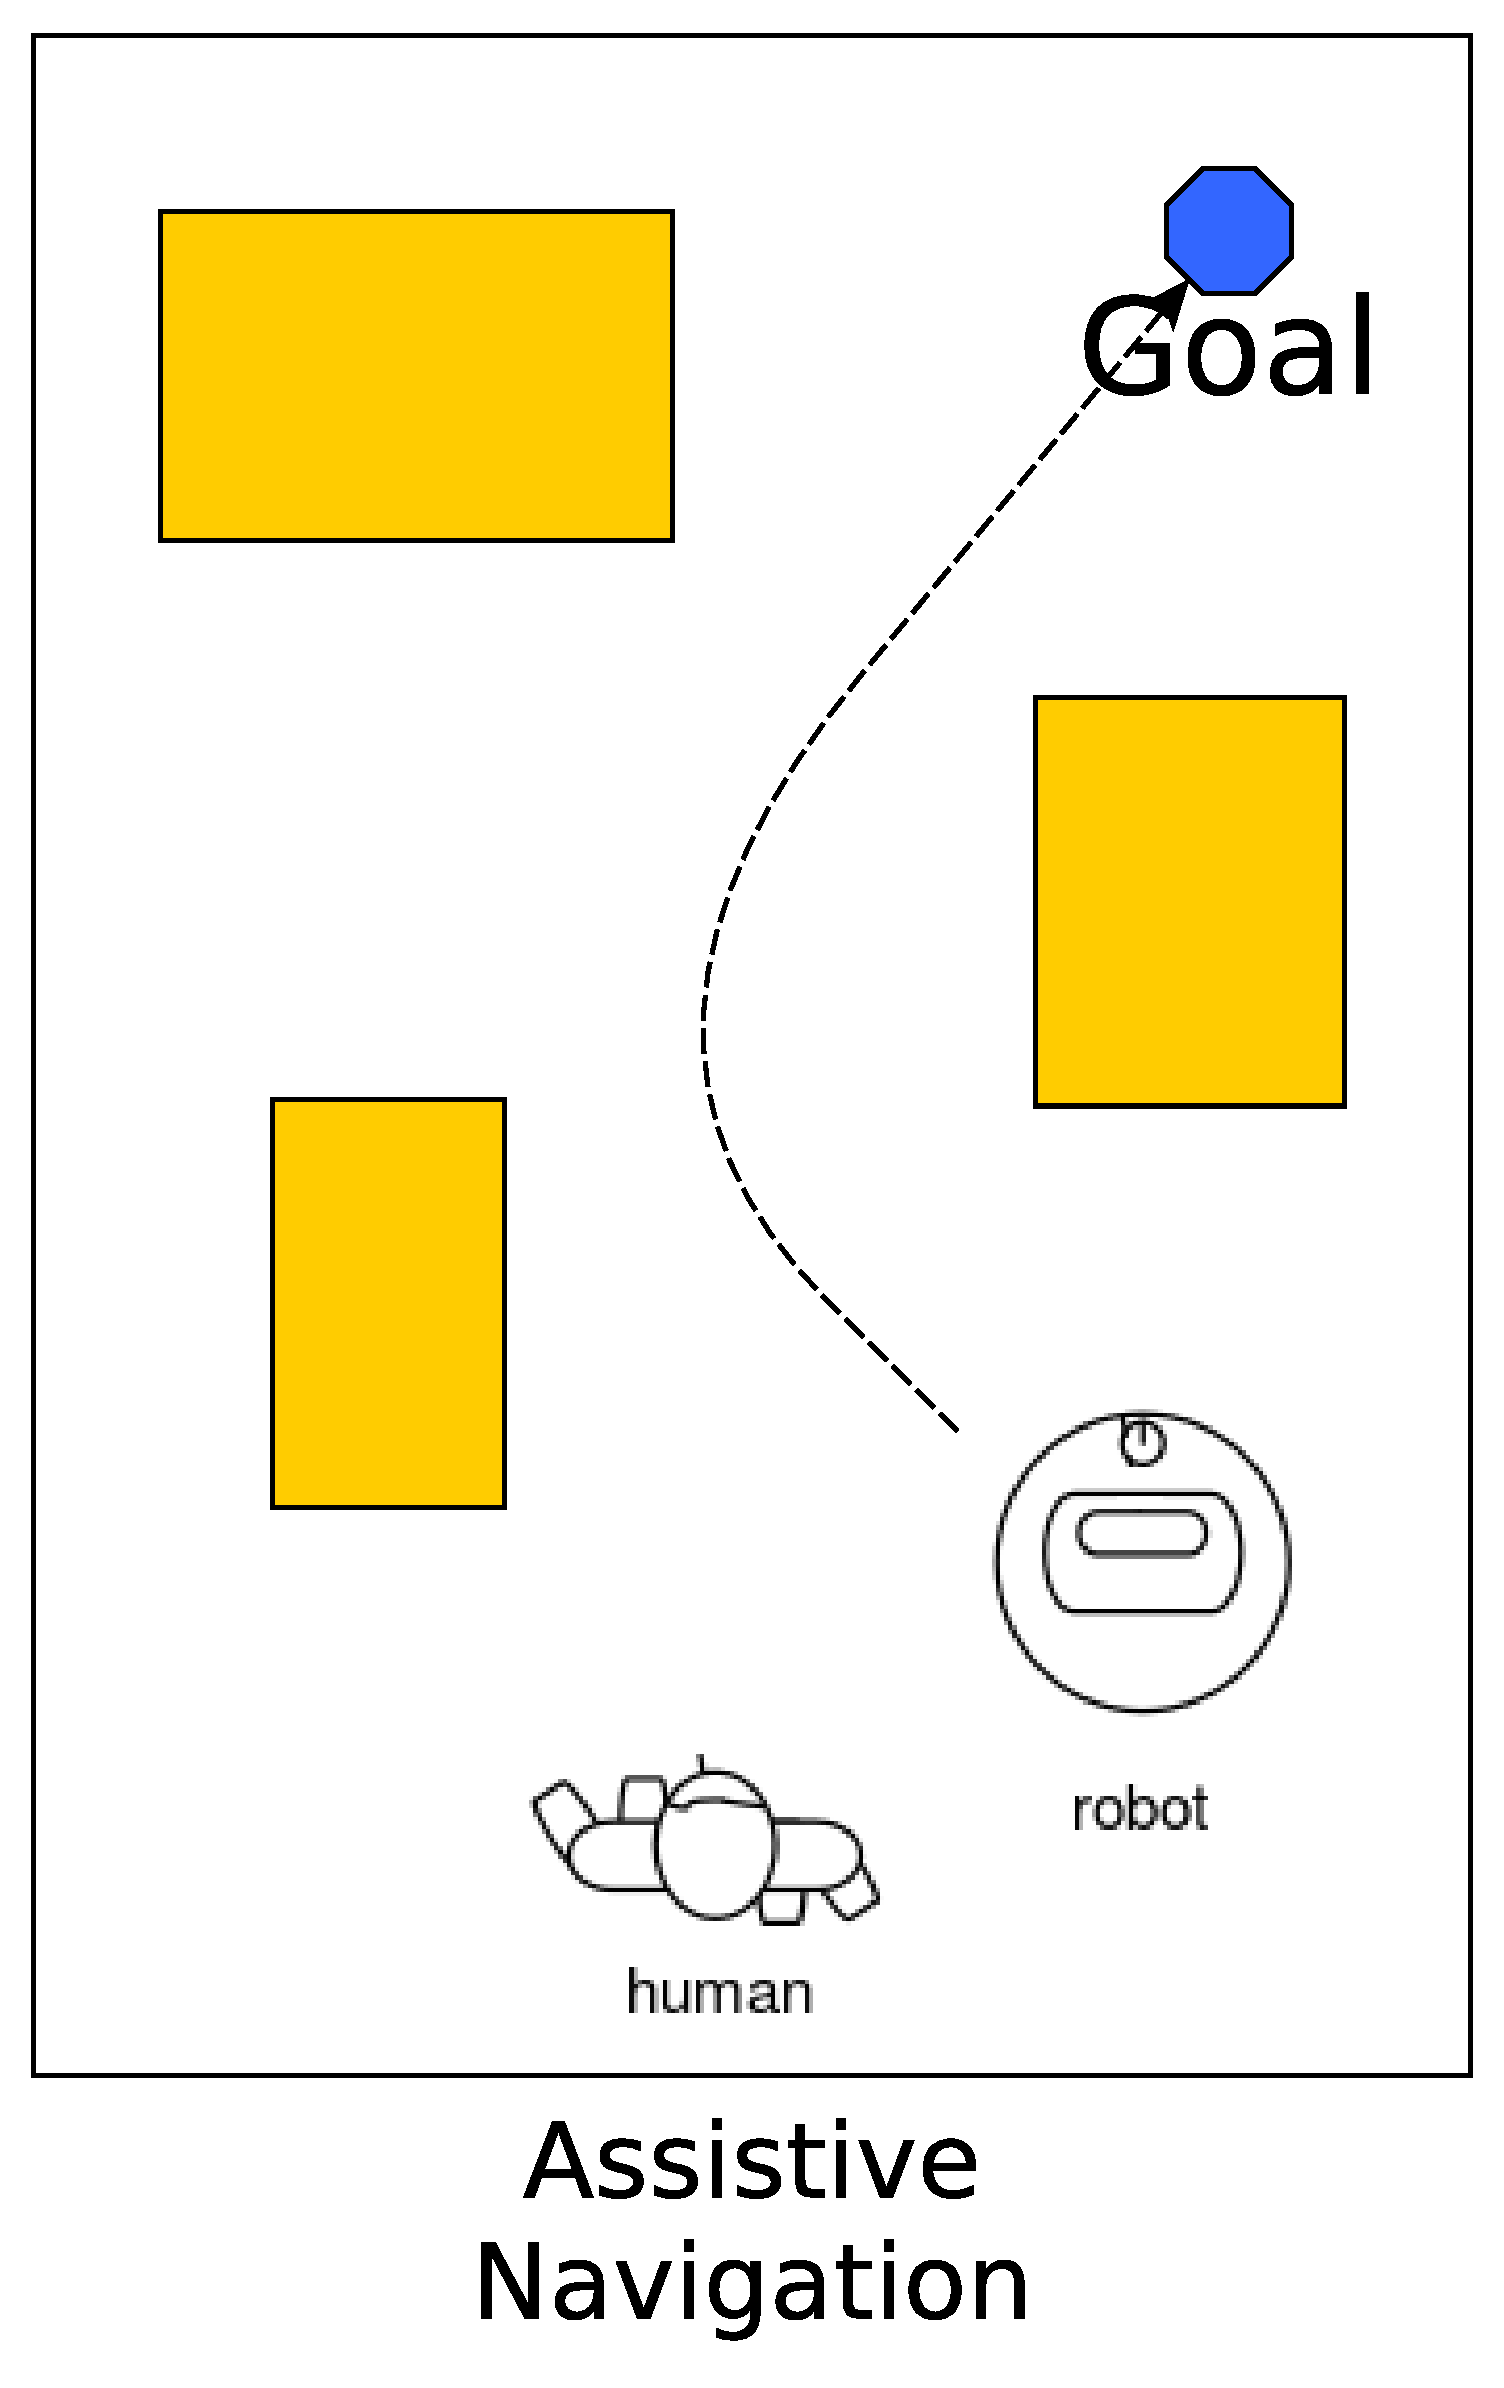
\includegraphics[width=.2\textwidth]{CasoAsistencia}
    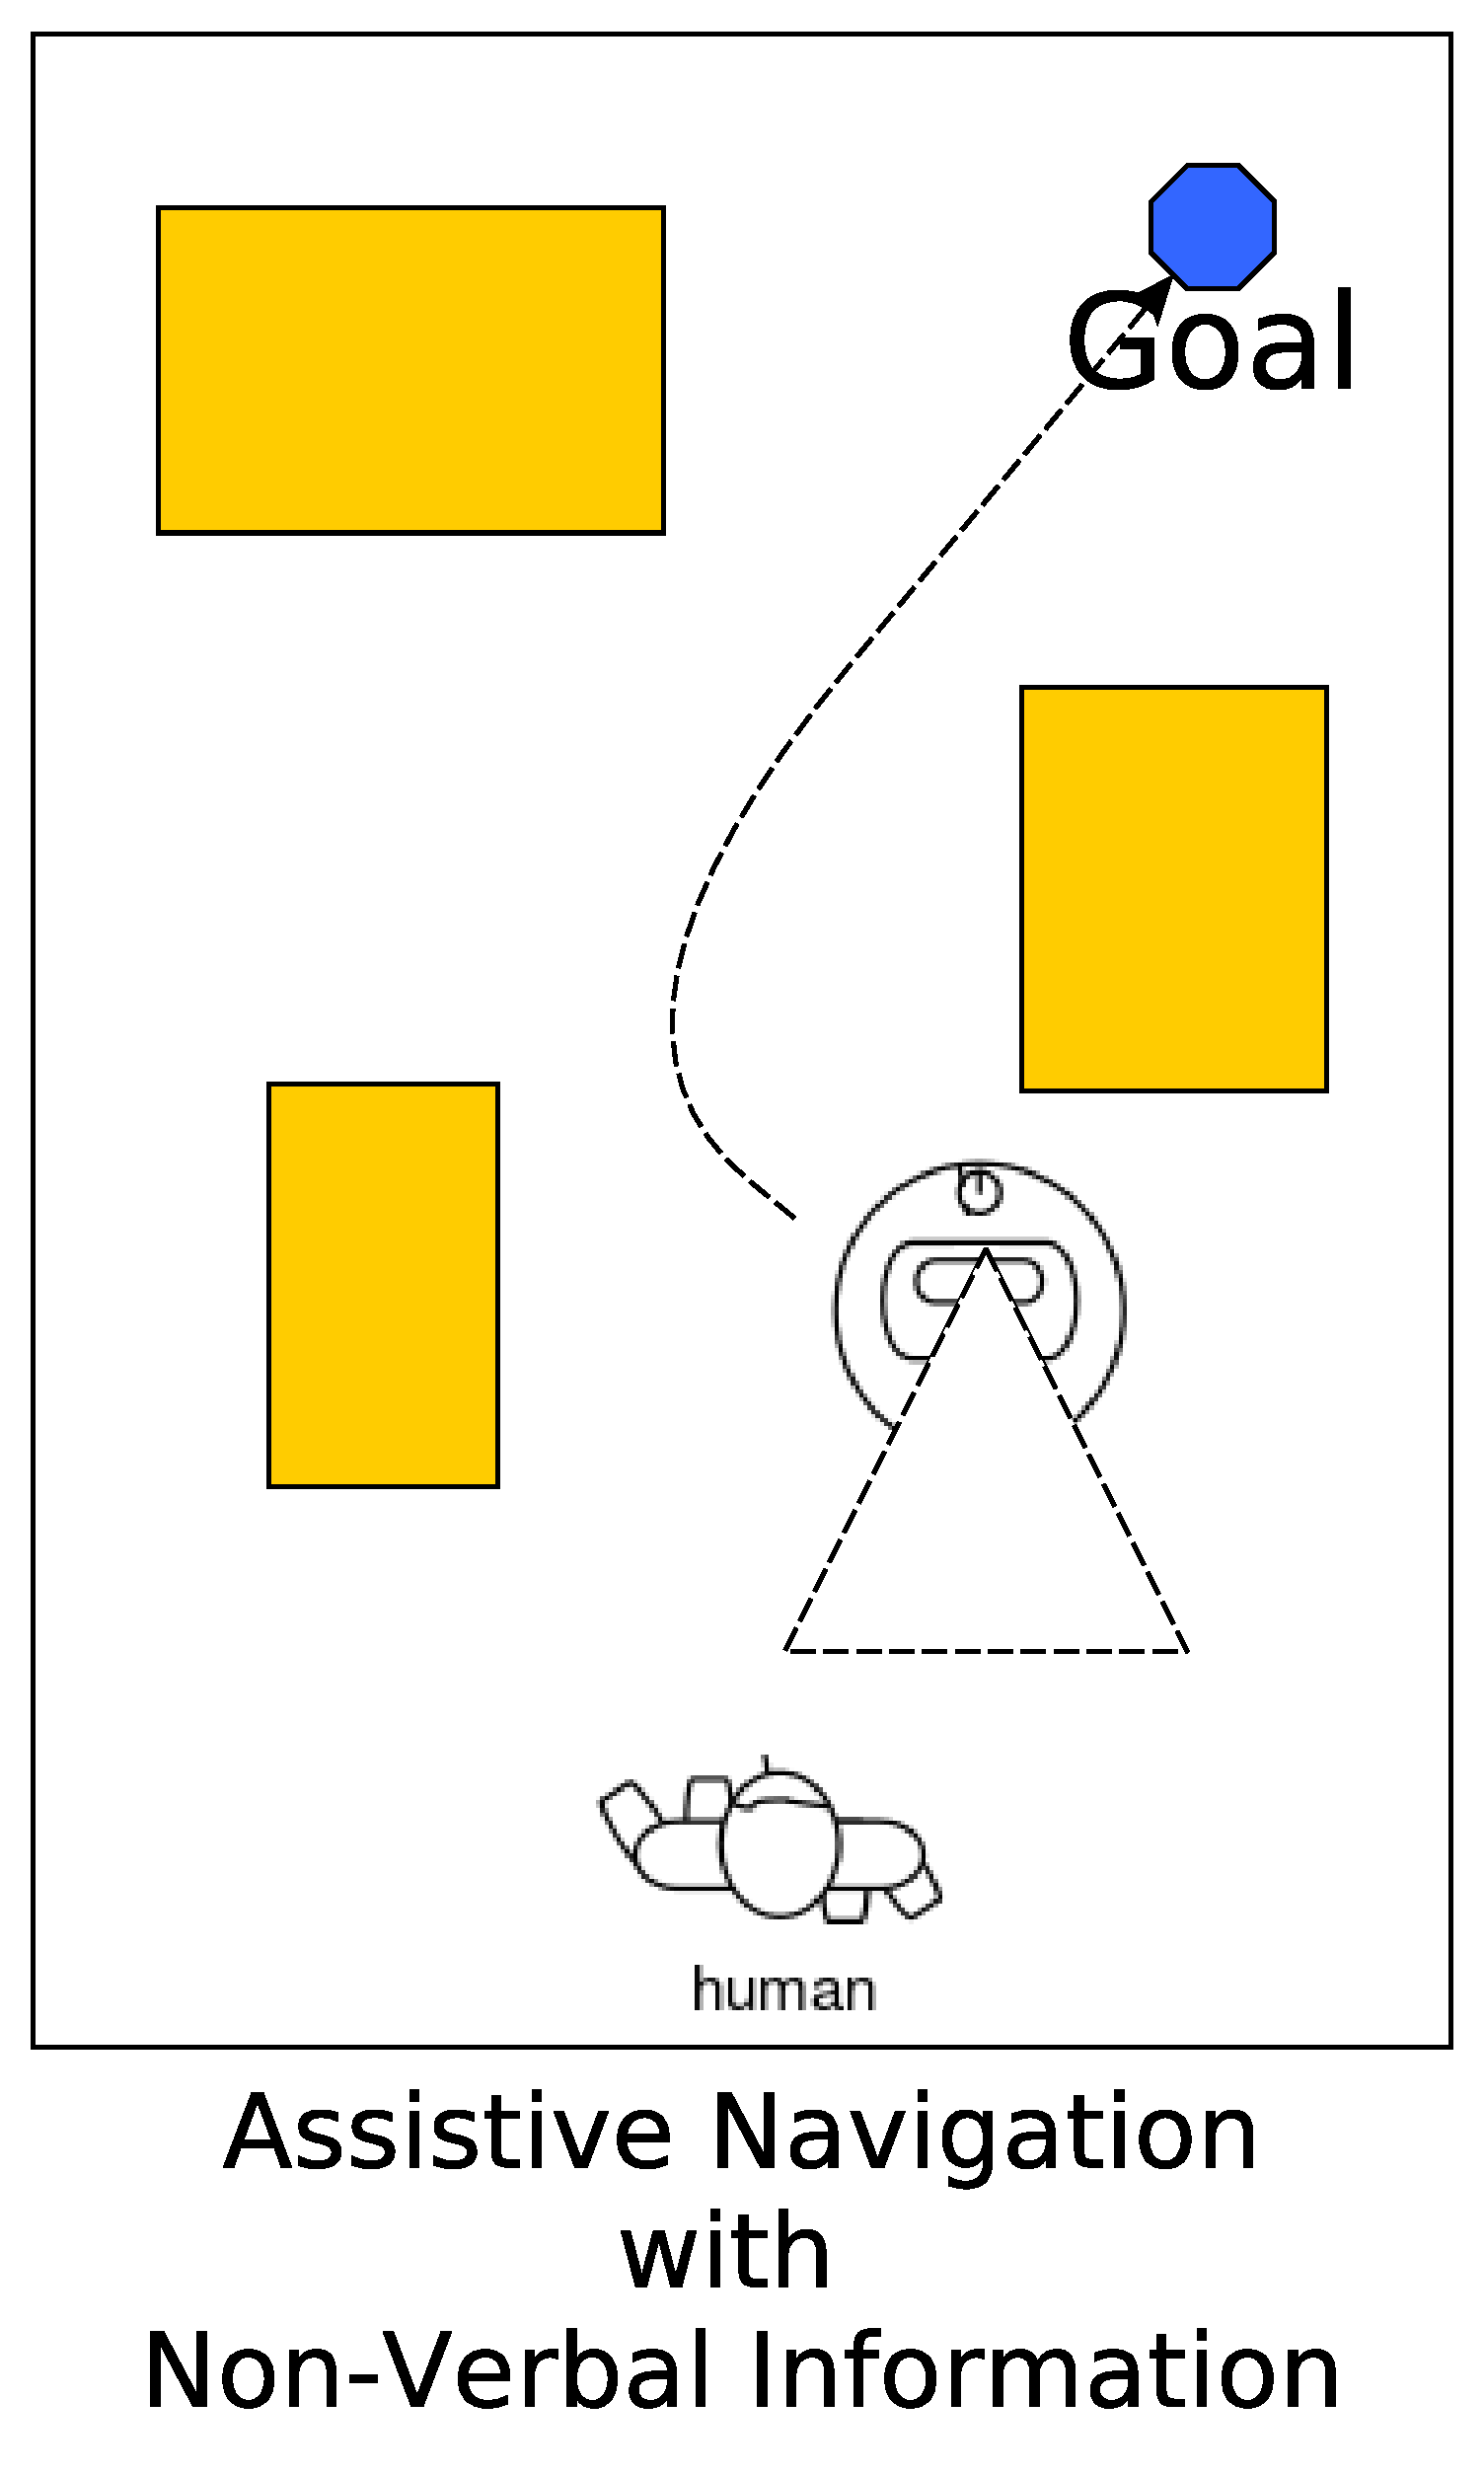
\includegraphics[width=.2\textwidth]{CasoAsistenciaNonVerbal}
%     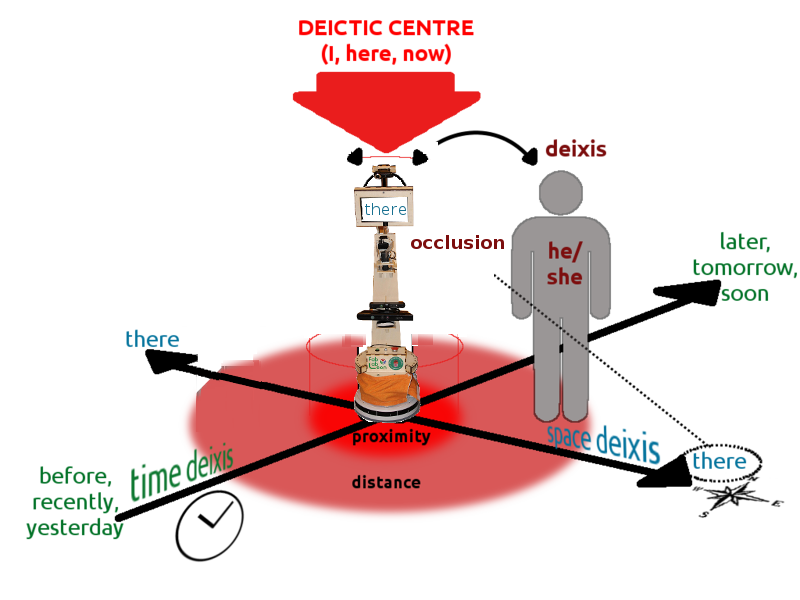
\includegraphics[width=.2\textwidth]{800px-Deixis2}
    \caption{Two methods of assistive tasks (attending the follow-me approach): guidance without users (non-follow-me), 
    guidance with disregarded users (follow-me without attention) and 
    guidance with attended users offering non-verbal information to user (follow-me with attention).}
  \label{fig:socialnavigation}
\end{figure}



\section{Reusability}

Poner el repo de githuba de PACO, poner el repo de GitHub del equipo.



\section{Conclusions and Future Work}

% % % % \medskip\noindent{\itshape Sample Output}
% % % % \begin{table}
% % % % \caption{Critical $N$ values}
% % % % \begin{center}
% % % % \renewcommand{\arraystretch}{1.4}
% % % % \setlength\tabcolsep{3pt}
% % % % \begin{tabular}{llllll}
% % % % \hline\noalign{\smallskip}
% % % % ${\mathrm M}_\odot$ & $\beta_{0}$ & $T_{\mathrm c6}$ & $\gamma$
% % % %   & $N_{\mathrm{crit}}^{\mathrm L}$
% % % %   & $N_{\mathrm{crit}}^{\mathrm{Te}}$\\
% % % % \noalign{\smallskip}
% % % % \hline
% % % % \noalign{\smallskip}
% % % %  30 & 0.82 & 38.4 & 35.7 & 154 & 320 \\
% % % %  60 & 0.67 & 42.1 & 34.7 & 138 & 340 \\
% % % % 120 & 0.52 & 45.1 & 34.0 & 124 & 370 \\
% % % % \hline
% % % % \end{tabular}
% % % % \end{center}
% % % % \end{table}
% % % % 
% % % % Before continuing your text you need an empty line. \dots
% % % % 
% % % % \vspace{3mm}
% % % % For further information you will find a complete description of
% % % % the tabular environment
% % % % on p.~62~ff. and p.~204 of the {\em \LaTeX{} User's Guide \& Reference
% % % % Manual\/} by Leslie Lamport.
% % % % %
% % % % \subsection{Tables Not Coded with \protect\LaTeX{}}
% % % % %
% % % % If you do not wish to code your table using \LaTeX{}
% % % % but prefer to have it reproduced separately,
% % % % proceed as for figures and use the following coding:\\[2mm]
% % % % {\itshape Sample Input}
% % % % \begin{verbatim}
% % % % \begin{table}
% % % % \caption{text of your caption}
% % % % \vspace{x cm}     % the actual height needed for your table
% % % % \end{table}
% % % % \end{verbatim}
% % % % %
% % % % \subsection{Signs and Characters}
% % % % %
% % % % \subsubsection*{Special Signs.}
% % % % %
% % % % You may need to use special signs.  The available ones are listed in the
% % % % {\em \LaTeX{} User's Guide \& Reference Manual\/} by Leslie Lamport,
% % % % pp.~41\,ff.
% % % % We have created further symbols for math mode (enclosed in \$):
% % % % \begin{center}
% % % % \begin{tabular}{l@{\hspace{1em}yields\hspace{1em}}
% % % % c@{\hspace{3em}}l@{\hspace{1em}yields\hspace{1em}}c}
% % % % \verb|\grole| & $\grole$ & \verb|\getsto| & $\getsto$\\
% % % % \verb|\lid|   & $\lid$   & \verb|\gid|    & $\gid$
% % % % \end{tabular}
% % % % \end{center}
% % % % %
% % % % \subsubsection*{Gothic (Fraktur).}
% % % % %
% % % % If gothic letters are {\itshape necessary}, please use those of the
% % % % relevant \AmSTeX{} alphabet which are available using the amstex
% % % % package of the American Mathematical Society.
% % % % 
% % % % In \LaTeX{} only the following gothic letters are available:
% % % % \verb|$\Re$| yields $\Re$ and \verb|$\Im$| yields $\Im$. These should
% % % % {\itshape not\/} be used when you need gothic letters for your contribution.
% % % % Use \AmSTeX{} gothic as explained above. For the real and the imaginary
% % % % parts of a complex number within math mode you should use instead:
% % % % \verb|$\mathrm{Re}$| (which yields Re) or \verb|$\mathrm{Im}$| (which
% % % % yields Im).
% % % % %
% % % % \subsubsection*{Script.}
% % % % %
% % % % For script capitals use the coding
% % % % \begin{center}
% % % % \begin{tabular}{l@{\hspace{1em}which yields\hspace{1em}}c}
% % % % \verb|$\mathcal{AB}$| & $\mathcal{AB}$
% % % % \end{tabular}
% % % % \end{center}
% % % % (see p.~42 of  the \LaTeX{} book).
% % % % %
% % % % \subsubsection*{Special Roman.}
% % % % %
% % % % If you need other symbols than those below, you could use
% % % % the blackboard bold characters of \AmSTeX{},  but there might arise
% % % % capacity problems
% % % % in loading additional \AmSTeX{} fonts. Therefore  we created
% % % % the blackboard bold characters listed below.
% % % % Some of them are not esthetically
% % % % satisfactory. This need not deter you from using them:
% % % % in the final printed form they will be
% % % % replaced by the well-designed MT (monotype) characters of
% % % % the phototypesetting machine.
% % % % \begin{flushleft}
% % % % \begin{tabular}{@{}ll@{ yields }
% % % % c@{\hspace{1.em}}ll@{ yields }c}
% % % % \verb|\bbbc| & (complex numbers)   & $\bbbc$
% % % %   & \verb|\bbbf| & (blackboard bold F) & $\bbbf$\\
% % % % \verb|\bbbh| & (blackboard bold H) & $\bbbh$
% % % %   & \verb|\bbbk| & (blackboard bold K) & $\bbbk$\\
% % % % \verb|\bbbm| & (blackboard bold M) & $\bbbm$
% % % %   & \verb|\bbbn| & (natural numbers N) & $\bbbn$\\
% % % % \verb|\bbbp| & (blackboard bold P) & $\bbbp$
% % % %   & \verb|\bbbq| & (rational numbers)  & $\bbbq$\\
% % % % \verb|\bbbr| & (real numbers)      & $\bbbr$
% % % %   & \verb|\bbbs| & (blackboard bold S) & $\bbbs$\\
% % % % \verb|\bbbt| & (blackboard bold T) & $\bbbt$
% % % %   & \verb|\bbbz| & (whole numbers)     & $\bbbz$\\
% % % % \verb|\bbbone| & (symbol one)      & $\bbbone$
% % % % \end{tabular}
% % % % \end{flushleft}
% % % % \begin{displaymath}
% % % % \begin{array}{c}
% % % % \bbbc^{\bbbc^{\bbbc}} \otimes
% % % % \bbbf_{\bbbf_{\bbbf}} \otimes
% % % % \bbbh_{\bbbh_{\bbbh}} \otimes
% % % % \bbbk_{\bbbk_{\bbbk}} \otimes
% % % % \bbbm^{\bbbm^{\bbbm}} \otimes
% % % % \bbbn_{\bbbn_{\bbbn}} \otimes
% % % % \bbbp^{\bbbp^{\bbbp}}\\[2mm]
% % % % \otimes
% % % % \bbbq_{\bbbq_{\bbbq}} \otimes
% % % % \bbbr^{\bbbr^{\bbbr}} \otimes
% % % % \bbbs^{\bbbs_{\bbbs}} \otimes
% % % % \bbbt^{\bbbt^{\bbbt}} \otimes
% % % % \bbbz \otimes
% % % % \bbbone^{\bbbone_{\bbbone}}
% % % % \end{array}
% % % % \end{displaymath}
% % % % %
% % % % \section{References}
% % % % \label{refer}
% % % % %
% % % % There are three reference systems available; only one, of course,
% % % % should be used for your contribution. With each system (by
% % % % number only, by letter-number or by author-year) a reference list
% % % % containing all citations in the
% % % % text, should be included at the end of your contribution placing the
% % % % \LaTeX{} environment \verb|thebibliography| there.
% % % % For an overall information on that environment
% % % % see the {\em \LaTeX{} User's Guide \& Reference
% % % % Manual\/} by Leslie Lamport, p.~71.
% % % % 
% % % % There is a special {\sc Bib}\TeX{} style for LLNCS that works along
% % % % with the class: \verb|splncs.bst|
% % % % -- call for it with a line \verb|\bibliographystyle{splncs}|.
% % % % If you plan to use another {\sc Bib}\TeX{} style you are customed to,
% % % % please specify the option \verb|[oribibl]| in the
% % % % \verb|documentclass| line, like:
% % % % \begin{verbatim}
% % % % \documentclass[oribibl]{llncs}
% % % % \end{verbatim}
% % % % This will retain the original \LaTeX{} code for the bibliographic
% % % % environment and the \verb|\cite| mechanism that many {\sc Bib}\TeX{}
% % % % applications rely on.
% % % % %
% % % % \subsection{References by Letter-Number or by Number Only}
% % % % %
% % % % References are cited in the text -- using the \verb|\cite|
% % % % command of \LaTeX{} -- by number or by letter-number in square
% % % % brackets, e.g.\ [1] or [E1, S2], [P1], according to your use of the
% % % % \verb|\bibitem| command in the \verb|thebibliography| environment. The
% % % % coding is as follows: if you choose your own label for the sources by
% % % % giving an optional argument to the \verb|\bibitem| command the citations
% % % % in the text are marked with the label you supplied. Otherwise a simple
% % % % numbering is done, which is preferred.
% % % % \begin{verbatim}
% % % % The results in this section are a refined version
% % % % of \cite{clar:eke}; the minimality result of Proposition~14
% % % % was the first of its kind.
% % % % \end{verbatim}
% % % % The above input produces the citation: ``\dots\ refined version of
% % % % [CE1]; the min\-i\-mality\dots''. Then the \verb|\bibitem| entry of
% % % % the \verb|thebibliography| environment should read:
% % % % \begin{verbatim}
% % % % \begin{thebibliography}{[MT1]}
% % % % .
% % % % .
% % % % \bibitem[CE1]{clar:eke}
% % % % Clarke, F., Ekeland, I.:
% % % % Nonlinear oscillations and boundary-value problems for
% % % % Hamiltonian systems.
% % % % Arch. Rat. Mech. Anal. 78, 315--333 (1982)
% % % % .
% % % % .
% % % % \end{thebibliography}
% % % % \end{verbatim}
% % % % The complete bibliography looks like this:
% % % % %
% % % % \begin{thebibliography}{[MT1]}
% % % % %
% % % % \bibitem[CE1]{clar:eke}
% % % % Clarke, F., Ekeland, I.:
% % % % Nonlinear oscillations and
% % % % boundary-value problems for Hamiltonian systems.
% % % % Arch. Rat. Mech. Anal. 78, 315--333 (1982)
% % % % %
% % % % \bibitem[CE2]{clar:eke:2}
% % % % Clarke, F., Ekeland, I.:
% % % % Solutions p\'{e}riodiques, du
% % % % p\'{e}riode donn\'{e}e, des \'{e}quations hamiltoniennes.
% % % % Note CRAS Paris 287, 1013--1015 (1978)
% % % % %
% % % % \bibitem[MT1]{mich:tar}
% % % % Michalek, R., Tarantello, G.:
% % % % Subharmonic solutions with prescribed minimal
% % % % period for nonautonomous Hamiltonian systems.
% % % % J. Diff. Eq. 72, 28--55 (1988)
% % % % %
% % % % \bibitem[Ta1]{tar}
% % % % Tarantello, G.:
% % % % Subharmonic solutions for Hamiltonian
% % % % systems via a $\bbbz_{p}$ pseudoindex theory.
% % % % Annali di Matematica Pura (to appear)
% % % % %
% % % % \bibitem[Ra1]{rab}
% % % % Rabinowitz, P.:
% % % % On subharmonic solutions of a Hamiltonian system.
% % % % Comm. Pure Appl. Math. 33, 609--633 (1980)
% % % % \end{thebibliography}
% % % % %
% % % % \subsubsection*{Number-Only System.}
% % % % %
% % % % For this preferred system do not use the optional argument
% % % % in the \verb|\bibitem| command: then, only numbers will
% % % % appear for the citations in the text (enclosed in square brackets)
% % % % as well as for the marks in your
% % % % bibliography (here the number is only end-punctuated without
% % % % square brackets).
% % % % 
% % % % Subsequent citation numbers in the text are collapsed to ranges.
% % % % Non-numeric and undefined labels are handled correctly but no sorting is
% % % % done.
% % % % 
% % % % E.g., \verb|\cite{n1,n3,n2,n3,n4,n5,foo,n1,n2,n3,?,n4,n5}| -- where
% % % % \verb|n|$x$ is the key of the $x^{\mathrm{th}}$ \verb|\bibitem|
% % % % command in sequence, \verb|foo| is the key of a \verb|\bibitem| with an
% % % % optional argument, and \verb|?| is an undefined reference -- gives
% % % % 1,3,2-5,foo,1-3,?,4,5 as the citation reference.
% % % % 
% % % % \begin{verbatim}
% % % % \begin{thebibliography}{1}
% % % % \bibitem {clar:eke}
% % % % Clarke, F., Ekeland, I.:
% % % % Nonlinear oscillations and boundary-value problems for
% % % % Hamiltonian systems.
% % % % Arch. Rat. Mech. Anal. 78, 315--333 (1982)
% % % % \end{thebibliography}
% % % % \end{verbatim}
% % % % %
% % % % \subsection{Author-Year System}
% % % % %
% % % % References are cited in the text by name and year in parentheses
% % % % and should look as follows:
% % % % (Smith 1970, 1980), (Ekeland et al. 1985, Theorem 2), (Jones and Jaffe
% % % % 1986; Farrow 1988, Chap.\,2). If the name is part of the sentence
% % % % only the year may appear in parentheses,
% % % % e.g.\ Ekeland et al. (1985, Sect.\,2.1)
% % % % The reference list should contain all citations occurring in the text,
% % % % ordered alphabetically by surname (with initials following). If there
% % % % are several works by the same author(s) the references should be listed
% % % % in the appropriate order indicated below:
% % % % \begin{alpherate}
% % % % \setlength{\hfuzz}{5pt}
% % % % \item
% % % % One author: list works chronologically;
% % % % \item
% % % % Author and same co-author(s): list works chronologically;
% % % % \item
% % % % Author and different co-authors: list works alphabetically
% % % % according to co-authors.
% % % % \end{alpherate}
% % % % If there are several works by the same author(s) and in the same year,
% % % % but which are cited separately, they should be distinguished by the use
% % % % of ``a'', ``b'' etc., e.g.\ (Smith 1982a), (Ekeland et al. 1982b).
% % % % %
% % % % \subsubsection*{How to Code Author-Year System.}
% % % % %
% % % % If you want to use this system you have to specify the option
% % % % \verb|[citeauthoryear]| in the \verb|documentclass|, like:
% % % % \begin{verbatim}
% % % % \documentclass[citeauthoryear]{llncs}
% % % % \end{verbatim}
% % % % Write your citations in the text explicitly except for the year, leaving
% % % % that up to \LaTeX{} with the \verb|\cite| command. Then give only the
% % % % appropriate year as the optional argument (i.e. the label in square
% % % % brackets) with the \verb|\bibitem| command(s).\\[2mm]
% % % % {\itshape Sample Input}
% % % % \begin{verbatim}
% % % % The results in this section are a refined version
% % % % of Clarke and Ekeland (\cite{clar:eke}); the minimality result of
% % % % Proposition~14 was the first of its kind.
% % % % \end{verbatim}
% % % % The above input produces the citation: ``\dots\ refined version of
% % % % Clarke and Ekeland (1982); the minimality\dots''. Then the
% % % % \verb|\bibitem| entry of \verb|clar:eke| in the \verb|thebibliography|
% % % % environment should read:
% % % % \begin{verbatim}
% % % % \begin{thebibliography}{}  % (do not forget {})
% % % % .
% % % % .
% % % % \bibitem[1982]{clar:eke}
% % % % Clarke, F., Ekeland, I.:
% % % % Nonlinear oscillations and boundary-value problems for
% % % % Hamiltonian systems.
% % % % Arch. Rat. Mech. Anal. 78, 315--333 (1982)
% % % % .
% % % % .
% % % % \end{thebibliography}
% % % % \end{verbatim}
% % % % {\itshape Sample Output}

\bibliographystyle{splncs03}
% argument is your BibTeX string definitions and bibliography database(s)
\bibliography{biblio}
% \bibauthoryear
%
\newpage

\section{Team Description}

\begin{itemize}

  \item Team name: RB1
  \item Contact information: 
  \item Website: robotica.unileon.es
  \item Team members:
      \begin{itemize}
	\item Francisco Lera
	\item Fernando Garc�a
	\item Jes�s Balsa
	\item Vicente Matell�n
	\item Franciso Mart�n
      \end{itemize}
  
\end{itemize}

\section{Hardware Description}

\begin{itemize}

  \item Robot name: RB1
  \begin{enumerate}
    \item Base:
    
    \item Vision Sensors: RGB-D Xtion
    \item Range sensors: Frontal laser 
    \item Dialogue Sensors: Directional microphone Rode Rycote , Loudspeakers
    \item Manipulation: 7DOF arm. Dynamixel Pro servos. Workspace: 70 cm
    \item Computer Description: Intel Core i7 with 8 GB of RAM and a 200 GB of disk
    \item Torso: +40
    \item Head: pan-tilt head.
  \end{enumerate}

\end{itemize}


\section{Software Description}

\begin{itemize}
 \item Development framework: ROS
  \begin{enumerate}
   \item Paquete
   \item Paquete
   \item Paquete
   \item Paquete
   \item Paquete
   \item Paquete
  \end{enumerate}


  \item Robot Control: Bica 
\end{itemize}




\end{document}
